\newpage
\section{Creating a line of signs: \tkzcname{tkzTabLine}}
\subsection{Definition}

\begin{NewMacroBox}{tkzTabLine}{\oarg{local options}\var{s(1),...,s(2n-1)}}
  $n$ is the number of elements of the second argument of \tkzname{tkzTabInit}.

\medskip
\begin{tabular}{lll}
\toprule
symbol in an odd position &  & definition \\
\midrule
\TAline{z} {}  {draws a dotted rule with a centered zero}
\TAline{t} {}  {draws a centered dotted rule}
\TAline{d} {}  {draws a centered double bar}
\TAline{\BS textvisiblespace}{} {nothing }
\bottomrule
\end{tabular}

\medskip
\begin{tabular}{lll}
\toprule
symbol in an even position & & definition                   \\
\midrule
\TAline{h}  {}  {forbidden zone}
\TAline{+}  {}  {the sign $+$}
\TAline{-}  {}  {the sign $-$}
\TAline{\BS textvisiblespace}{} {nothing }
\bottomrule

\end{tabular}


\medskip
\noindent\emph{\tkzcname{tkzTabLine} takes as argument a list of symbols. In \tkzname{normal} use, the symbols belong to two categories: symbols in odd positions and symbols in even positions. Symbols in odd positions are usually rules, and symbols in even positions are usually ``$+$ or $-$'' signs. Symbols in odd positions act graphically: they draw vertical rules. If the second argument of \tkzcname{tkzTabInit} has \textcolor{red}{$n$} elements (values of the variable), the argument of \tkzcname{tkzTabLine} contains \tkzname{$n$} of them. Symbols in even positions give a ``$+$ or $-$'' sign or a forbidden zone (hatched or colored). Each line of signs contains \tkzname{$n-1$} of them, so it has \tkzname{$2n-1$} elements in all, that is \tkzname{$2n-2$} commas!\\
The ``recognized'' symbols are given in the tables above, but you can put almost anything. Be careful, however: the comma \textcolor{red}{(,)} is the list separator, so a decimal number written with a comma must be protected. You have several possibilities:
\begin{itemize}
\item[--] \{4,5\}: put the number between braces.
\item[--] \tkzcname{numprint\{4,5\}} or \tkzcname{np\{4,5\}}, with the excellent package \tkzname{numprint}\NamePack{numprint}, loaded with the option \tkzname{np} for the shortcut.
\end{itemize}}

\medskip
\begin{tabular}{lllc}
\toprule
options   & default       & definition         \\
\midrule
\TOline{style}  {dotted    } {style of the vertical rules               }
\TOline{help}   {no default} {shows the structure of a line of signs     }
\bottomrule
\end{tabular}

\medskip
\noindent\emph{The style of the vertical rules can be changed locally, and you can get information about the structure of the line.}
\end{NewMacroBox}

\subsection{Number of arguments}
The general syntax is:

\begin{tkzltxexample}[]
 \tkzTabInit{ e(1),...,e(i),...,e(p)} % table with p rows
            { a(1),...,a(i),...,a(n)} % n values
 \tkzTabLine{ s(1),...,s(i),...,s(2n-1)}
\end{tkzltxexample}


\medskip
If the first row has \tkzname{$n$} values, there are \tkzname{$n$} symbols in odd positions and \tkzname{$n-1$} symbols in even positions, that is \tkzname{$2n-1$} symbols.

 The main symbols are: \tkzname{z} for a zero placed on a rule, \tkzname{t} for a rule matching a zero of another row, and \tkzname{d} for a value where the expression is not defined.

A simple illustration: three values $a_1$, $a_2$ and $a_3$ allow $2\times3 -1 =5$ symbols. With $3$ values in the first row, the argument of \tkzcname{tkzTabLine} must have {$2\times 3-1=5$} elements: a list of $3$ symbols in odd positions and $2$ symbols in even positions, that is $5$ symbols separated by $4$ commas.

\begin{center}
  \begin{tikzpicture}
    \tkzTabInit[espcl=3,lgt=2]%
    {\colorbox{red!40}{\textcolor{white}{$x$}}    / 1,%
     \colorbox{red!40}{\textcolor{white}{$f(x)$}} / 1}%
    {\colorbox{blue!40}{\textcolor{white}{ $a_1$}},%
     \colorbox{blue!40}{\textcolor{white}{ $a_2$}},%
     \colorbox{blue!40}{\textcolor{white}{ $a_3$}}}%
    \path (N11)--(N12) node[circle,draw, fill= lightgray,midway] {1};
    \path (N12)--(N21) node[midway] {$,$};
    \path (N21)--(N22) node[circle, draw, fill= lightgray,midway] {3};
    \path (N31)--(N32) node[circle,draw,  fill= lightgray,midway] {5};
    \path (M11)--(M12) node[circle, draw, fill= orange!30,midway] {2};
    \path (M21)--(M22) node[circle,draw,  fill= orange!30,midway] {4};
  \end{tikzpicture}
\end{center}

To get this line, enter
\begin{tkzexample}[code only]\tkzTabLine{ $1$ , $2$ , $3$ , $4$ , $5$}
\end{tkzexample}


\subsection{Minimal use}
The second row is empty, but the argument of \tkzcname{tkzTabLine} must contain \tkzname{$4$} commas: it is a list of \tkzname{$5 = 2\times3-1$} values.

\begin{tkzexample}[code only]
 \tkzTabLine{,,,,} or \tkzTabLine{ , , , , }\end{tkzexample}

\begin{tkzexample}[width=8cm,small]
\begin{tikzpicture}
  \tkzTabInit[espcl=1.5]
     {$x$  / 1 ,$f(x)$ /1 }%
     {$v_1$ , $v_2$ , $v_3$ }%
  \tkzTabLine{ , , , , }
\end{tikzpicture}
\end{tkzexample}

\subsubsection{\texttt{\textcolor{red}{t}}: adding a rule}
This symbol draws a simple vertical rule.
\begin{tkzexample}[width=8cm,small]
\begin{tikzpicture}
  \tkzTabInit[espcl=1.5]
     {$x$  / 1 ,$f(x)$ /1 }%
     {$v_1$ , $v_2$ , $v_3$ }%
  \tkzTabLine{ t, , t , ,t }
\end{tikzpicture}
\end{tkzexample}

\subsubsection{\texttt{\textcolor{red}{z}}: adding a zero on a vertical rule}
\begin{tkzexample}[width=8cm,small]
\begin{tikzpicture}
  \tkzTabInit[espcl=1.5]
     {$x$  / 1 ,$f(x)$ /1 }%
     {$v_1$ , $v_2$ , $v_3$ }%
  \tkzTabLine{ z, , z , ,z }
\end{tikzpicture}
\end{tkzexample}

\subsubsection{\texttt{\textcolor{red}{d}}: double bar}

A function may be undefined at $0$ and at $2$ and vanish at $1$. Put the symbol |d| at each end.

\begin{tkzexample}[width=7cm,small]
\begin{tikzpicture}
  \tkzTabInit[espcl=1.5]%
    {$x$ / 1,$g(x)$ / 1}%
    {$0$,$1$,$2$}%
\tkzTabLine{d,+,0,-,d}
\end{tikzpicture}
\end{tkzexample}

A function may also have a right derivative different from its left derivative.

\begin{tkzexample}[width=7cm,small]
\begin{tikzpicture}
   \tkzTabInit[lgt=1.5,espcl=1.75]%
       {$x$ / 1,$f'(x)$ / 1}%
       {$-\infty$,$0$,$+\infty$}%
   \tkzTabLine{,+,d,-,}
\end{tikzpicture}
\end{tkzexample}

\subsection{Using the symbols in even positions}

In a table of signs, the symbols in even positions are normally signs, but the macro can be used in other ways. The next example shows a classic case: a zone of the table that corresponds to forbidden values. By default, with the symbol \tkzname{h}, the zone is gray, but it can be hatched if you prefer.
The last example shows how to use the macro in another way.

\subsubsection{\texttt{\textcolor{red}{h}}: forbidden zone}

A function may be undefined on an interval, here $[1, 2]$. The part of the table that corresponds to this interval is hatched or colored (by default, the zone is gray). Put |h| between the two |d| that correspond to the forbidden values\index{forbidden values} $1$ and $2$.

\begin{tkzexample}[width=8cm, small]
\begin{tikzpicture}
  \tkzTabInit[color,espcl=1.5]
  {$x$ / 1,$g(x)$ / 1}
  {$0$,$1$,$2$,$3$}%
  \tkzTabLine{z, + , d , h , d , - , t}
\end{tikzpicture}
\end{tkzexample}

\subsection{Using the options}

\subsubsection{\tkzname{t style}: style of the vertical rules}
\Istyle{tkzTabLine}{t style}

\begin{tkzexample}[width=7cm, small]
\begin{tikzpicture}
\tikzset{t style/.style = {style = dashed}}
  \tkzTabInit[espcl=1.5]
     {$x$  / 1 ,$f(x)$ /1 }%
     {$v_1$ , $v_2$ , $v_3$ }%
  \tkzTabLine{ t, , t , ,t }
\end{tikzpicture}
\end{tkzexample}


\begin{tkzexample}[width=7cm, small]
\tikzset{t style/.style = {style = densely dashed}}
\begin{tikzpicture}
  \tkzTabInit[espcl=1.5]
     {$x$  / 1 ,$f(x)$ /1 }%
     {$v_1$ , $v_2$ , $v_3$ }%
  \tkzTabLine{ z, , z , ,z }
\end{tikzpicture}
\end{tkzexample}

\subsubsection{\tkzname{help}: shows the structure of the table}
\Iopt{tkzTabLine}{help}
See the section ``Customizing the tables'' (\ref{pers}).


\subsection{Using the styles}

\subsubsection{\tkzname{h style}: color of a forbidden zone}
\Istyle{tkzTabLine}{h style} \index{forbidden zone}
To color or hatch a zone of the table in another way, change a style.
\begin{tkzexample}[width=8cm,small]
\begin{tikzpicture}
  \tikzset{h style/.style = {fill=red!50}}
  \tkzTabInit[color,espcl=1.5]%
    {$x$ / 1,$g(x)$ / 1}%
    {$0$,$1$,$2$,$3$}%
  \tkzTabLine{z,+,d,h,d,-,t}
\end{tikzpicture}
\end{tkzexample}


This time the zone is hatched.
 \index{hatching}
\begin{tkzexample}[width=8cm,small]
\begin{tikzpicture}
  \tikzset{h style/.style =
          {pattern=north west lines}}
  \tkzTabInit[color,espcl=1.5]%
    {$x$ / 1,$g(x)$ / 1}%
    {$0$,$1$,$2$,$3$}%
  \tkzTabLine{z,+,,h,d,-,t}
\end{tikzpicture}
\end{tkzexample}



\subsection{Examples}

\subsubsection{Simplifying an expression with an absolute value}

\begin{tkzexample}[width=8cm,small]
 \begin{tikzpicture}
 \tkzTabInit[lgt=2,espcl=1.75]%
  {$x$/1,$2-x$/1, $\vert 2-x \vert $/1}%
  {$-\infty$,$2$,$+\infty$}%
 \tkzTabLine{ , + , z , - , }
 \tkzTabLine{ , 2-x ,z, x-2, }
\end{tikzpicture}
\end{tkzexample}

\subsubsection{Table of signs}

\begin{tkzexample}[ small]
\begin{tikzpicture}
  \tkzTabInit[lgt=3,espcl=1.5]%
     {$x$                                   /1,
      $x^2-3x+2$                            /1,
      $(x-\E)\ln x$                   /1,
      $\dfrac{x^2-3x+2}{(x-\E)\ln x}$ /2}
              {$0$  , $1$  , $2$  , $\E$  ,$+\infty$}
              \tkzTabLine{ t,+,z,-,z,+,t,+,}
              \tkzTabLine{ d,+,z,-,t,-,z,+,}
              \tkzTabLine{ d,+,d,+,z,-,d,+,}
\end{tikzpicture}
\end{tkzexample}


\subsubsection{Sign of a quadratic expression}

If $\Delta  \geq 0$, we can write $\displaystyle ax^2+bx+c=a\left(x-\dfrac{-b-\sqrt{b^2-4ac}}{2a}\right)\left(x-\dfrac{-b+\sqrt{b^2-4ac}}{2a}\right)$


\begin{tkzexample}[vbox,small]
\begin{tikzpicture}
 \tkzTabInit[color,lgt=5,espcl=3]%
   {$x$ / .8,$\Delta>0$\\ Sign of\\ $ax^2+bx+c$ /1.5}%
   {$-\infty$,$x_1$,$x_2$,$+\infty$}%
 \tkzTabLine{ , \genfrac{}{}{0pt}{0}{\text{sign of}}{a}, z
              , \genfrac{}{}{0pt}{0}{\text{opposite}}{\text{sign of}\ a}, z
              , \genfrac{}{}{0pt}{0}{\text{sign of}}{a},  }
 \end{tikzpicture}
\end{tkzexample}
 Note the use of the macro \tkzcname{genfrac}\footnote{\tkzcname{genfrac} is a macro of the package \tkzname{amsmath}}.

\medskip
If $\Delta  = 0$, we can write $\displaystyle ax^2+bx+c=a\left(x+\dfrac{b}{2a}\right)^2$

\begin{tkzexample}[vbox,width=7cm,small]
\begin{tikzpicture}
  \tkzTabInit[color,lgt=5,espcl=3]%
   {$x$ / 1 , $\Delta=0$\\ Sign of\\ $ax^2+bx+c$  / 2}%
   {$-\infty$,$\dfrac{-b}{2a}$,$+\infty$}%
  \tkzTabLine{ , \genfrac{}{}{0pt}{0}{\text{sign of}}{ a} , z
               , \genfrac{}{}{0pt}{0}{\text{sign of}}{a}, }
\end{tikzpicture}
\end{tkzexample}

If $\Delta  < 0$, then $\displaystyle ax^2+bx+c=a\left[\left(x+\dfrac{b}{2a}\right)^2 -\dfrac{b^2-4ac}{4a^2}\right]$

\begin{tkzexample}[vbox,width=7cm,small]
\begin{tikzpicture}
  \tkzTabInit[color,lgt=5,espcl=5]%
   {$x$/.8,$\Delta<0$\\ Sign of\\ $ax^2+bx+c$/2}%
   {$-\infty$,$+\infty$}%
 \tkzTabLine{ , \genfrac{}{}{0pt}{0}{\text{sign of}}{ a}, }
\end{tikzpicture}
\end{tkzexample}


\endinput
